\subsection{问题三：日内调整购电规划}\label{sec:q3}
\subsubsection{新增信息与交易变量}
问题三在固定电价下，每天00、06、12、18点可获得未来整点的光伏预报，并可在后三个时刻修订尚未交付的购电量。新预报有助于更新对光伏出力的判断，日内调整则可以结合实际库存和近期负荷重新安排购电。为判断两者各自的作用，后文在相同调整时刻下比较不同预报的使用效果。

记零时计划为$g_{d,t}$，发布时间对应的区间索引为$s\in\{0,36,72,108\}$，在$s$修订的剩余计划为$q^{(s)}_{d,t}$，最终交付的常规电量为$q_{d,t}$。规划根据预测安排购电，运行时仍按问题二的规则调节储能。可用信息$\mathcal H_{d,s}$包括此前日期的历史、当日$s$之前已完成区间的观测，以及截至$s$已发布的预报。

本问沿用余电可以不利用、原计划款不返还的假设。主要计算按每段最终交付量与零时计划的差额收费，允许撤回尚未交付的追加申报。下文将这一解释称为主合约，另比较追加电量成交后不可撤回、每笔分别收费的情形。

\subsubsection{费用目标与预报融合}
总费用由原计划、调整和紧急购电三项组成：
\begin{equation}
\begin{aligned}[b]
 C_3=\sum_{d,t}\bigl[&p_tg_{d,t}
 +1.5p_t(q_{d,t}-g_{d,t})_+\\
 &+0.5p_t(g_{d,t}-q_{d,t})_+
 +5p_te_{d,t}\bigr].
\end{aligned}\label{eq:netbill}
\end{equation}
其中$(x)_+=\max(x,0)$，求和覆盖正式期。增购1\,kWh额外支付$1.5p_t$；减购1\,kWh时，原计划款照付，另加$0.5p_t$违约费，即原价的50\%。

零时按$(\mathrm P_2)$制定计划，净负荷预测采用已发布预报与历史数据的融合结果。日内$s>0$时，原计划费用已经确定，因此重新规划以剩余时段的增购费用最小为目标：
\begin{equation}
 \min \widehat C_{3,d,s}=\sum_{t=s}^{143}1.5p_t\bigl(q^{(s)}_{d,t}-g_{d,t}\bigr).\label{eq:replan}
\end{equation}
本式采用$q^{(s)}_{d,t}\ge g_{d,t}$的约束，理由见下节。与问题二相同，未来紧急购电的风险通过净负荷分位修正来处理，实际费用则在运行后核算。

附件三中，$h$点发布的第$k$列预报对应$h+k$点。每次收到预报后，以最近一个已完成区间的光伏观测为插值起点，依次连接未来整点值，得到十分钟预测$\widehat P^{\mathrm{V,F}}$，并取其中截至当日24点的部分。

采用两来源线性融合：
\begin{equation}
 \widehat P^{\mathrm V}_{d,t}
 =(1-\lambda)\widehat P^{\mathrm{V,H}}_{d,t}
 +\lambda\widehat P^{\mathrm{V,F}}_{d,t},
 \qquad 0\le\lambda\le1.\label{eq:fusion}
\end{equation}
不同来源的预测误差可能相互补充，因而可通过组合改善预测\upcite{bates1969combination}，光伏预测中也已有自适应组合的研究\upcite{wei2026pv}。本文采用上述加权形式，并按实际购电费用选择权重，使预测效果能够通过最终支出评价。

为避免近期观测使预测水平发生过大跳变，先定义区间截断函数：
\begin{equation}
 \operatorname{clip}(x,a,b)=\min\{b,\max\{a,x\}\},\qquad a\le b.\label{eq:clip}
\end{equation}
其中$x$为待修正的数值，$a$、$b$分别为下限和上限：小于$a$时返回$a$，大于$b$时返回$b$，在区间内则保留$x$。本文将它作用于无量纲修正比例，例如$\operatorname{clip}(1.40,0.75,1.25)=1.25$。

在日内发布时刻$s\in\{36,72,108\}$，再用此前18个已完成区间，即最近3小时的观测修正负荷水平：
\begin{equation}
 \widehat P^{\mathrm L,(s)}_{d,t}
 =\widehat P^{\mathrm L}_{d,t}
 \operatorname{clip}\!\left(
 \frac{\overline{P^{\mathrm L}_{d,s-18:s}}}
      {\max(\overline{\widehat P^{\mathrm L}_{d,s-18:s}},1)},0.75,1.25
 \right),\quad t\ge s.
\end{equation}
横线表示索引$j=s-18,\ldots,s-1$上的算术均值，分母中的1以kW计，用于避免预测均值过小导致比值异常。该比值反映最近实际负荷与原预测的偏差。按式\eqref{eq:clip}限制在$[0.75,1.25]$后，每次修正幅度至多为原预测的25\%；上下限由控制规则设定，未作置信水平解释。将修正后的负荷与融合光伏相减，形成净负荷点预测，再按式\eqref{eq:risk}加入对应发布时间的历史残差分位。每种$\lambda$和预报组合分别计算残差，所用样本均来自此前日期。

\subsubsection{分条约束与汇总模型}
\textbf{a) 剩余时域供需平衡。}仅对$t\ge s$规划未来交付：
\begin{equation}
 q^{(s)}_{d,t}+\widehat b_{d,t}
 =\widetilde N^{(s)}_{d,t}+\widehat c_{d,t}+\widehat w_{d,t}.
\end{equation}
已交付区间不重新优化，其实际费用和库存变化均保留。

\textbf{b) 实际库存起点。}每次规划采用当时实际储电量，即$\widehat S_{d,s}=S_{d,s}$，并要求$\widehat S_{d,144}\ge6000$。预测中的储能运行继续满足问题一的状态递推、功率和库存限制。

\textbf{c) 原计划下界。}若某段$q<g$，可将$q$提高到$g$，差额计入未利用量。此时充放电和库存相同，还可省去减购违约费。因此，按主合约保留原计划量的费用更低，可加入
\begin{equation}
 q^{(s)}_{d,t}\ge g_{d,t},\qquad t\ge s.\label{eq:plan-floor}
\end{equation}
各次修订均以零时$g_t$为下界。此前的$q^{(s-36)}_t$中尚未交付的追加量可以撤回，费用最终按交付量与原计划的净差计算。

\textbf{d) 信息与动作时点。}本次$q^{(s)}$根据$\mathcal H_{d,s}$制定；此后各交付段获得的实际需求用于充放电反馈和紧急补购，已交付电量按当时计划记录。

省略日期下标，得到每次日内重规划的完整形式：
\begin{equation}
\begin{aligned}[b]
 (\mathrm P_3^{(s)})\quad\min\quad&
       \sum_{t=s}^{143}1.5p_t(q^{(s)}_t-g_t),\\
 \mathrm{s.t.}\quad&q^{(s)}_t+\widehat b_t
      =\widetilde N^{(s)}_t+\widehat c_t+\widehat w_t,\\
 &\widehat S_{t+1}=\widehat S_t+0.9\widehat c_t-\widehat b_t/0.9,\\
 &0\le\widehat c_t,\widehat b_t\le5000/6,\quad\widehat w_t\ge0,\quad q^{(s)}_t\ge g_t,\\
 &1200\le\widehat S_t\le10800,\quad
   \widehat S_s=S_{d,s},\quad\widehat S_{144}\ge6000.
\end{aligned}\label{eq:q3-summary}
\end{equation}
区间约束作用于$t=s,\ldots,143$，库存边界还包括144。剩余时域分别为108、72、36段，相应线性规划为540、360、180个连续变量。充放电互斥仍可按问题一的论证处理。

\subsubsection{求解与日内执行步骤}
权重候选为$\{0,0.25,0.50,0.75,1\}$，与六个分位组成30组参数。按1月15—31日实际费用比较，选得$(\lambda,\alpha)=(0.50,0.65)$。正式运行采用的1月热启动预先固定为纯附件三预测、0.80分位及三次日内调整，2月1日起使用所选参数。候选模拟仅用于评分，正式策略的初始库存由预先固定的热启动运行确定。

日前与日内协调优化已有相关研究\upcite{xiao2019mpc}。本问采用如下分时执行步骤：
\begin{enumerate}
 \item 零时继承真实库存，读取已发布光伏预报，与历史曲线融合并作风险修正，求解全天原计划$g$。
 \item 每到06、12、18点，接收本次新预报和此前已完成区间的负荷、光伏观测，更新剩余预测。
 \item 以当前实际库存为起点，求解$(\mathrm P_3^{(s)})$，更新尚未交付的常规计划，并记录各次修订。
 \item 在每个交付段以当前$q_t$替换问题二反馈式中的$g_t$，执行储能和必要的紧急购电。
 \item 根据最终$q_t-g_t$计算主合约调整费，日末将实际库存传至次日。
\end{enumerate}
日内LP给出当次预测下费用最低的常规计划，后续效果还取决于实际需求和储能反馈。因此，本问得到的是基于预测的可行调度策略。

\subsubsection{调度结果与费用来源}
正式期总费用为\PaperValue{q3-cost}\,元，比问题二减少\PaperValue{q3-saving}\,元，降幅\PaperValue{q3-saving-percent}\%。表\ref{tab:q3-comparison}将费用、电量和库存放在同一口径下比较。
\par
\begin{table}[!htbp]
\centering
\caption{固定电价下两种策略的结果（2—12月）}\label{tab:q3-comparison}
\normalsize
\begin{tabular}{lrr}
\toprule
\multicolumn{1}{c}{指标} & \multicolumn{1}{c}{零时固定计划} & \multicolumn{1}{c}{日内调整计划} \\
\midrule
原计划费/元 & 13,291,625.72 & 12,649,467.17 \\
调整费/元 & 0.00 & 527,937.93 \\
紧急费/元 & 616,550.23 & 138,430.89 \\
总费用/元 & 13,908,175.95 & 13,315,835.99 \\
常规购电/kWh & 21,712,548.31 & 21,197,074.02 \\
紧急购电/kWh & 102,787.48 & 25,862.57 \\
未利用电量/kWh & 2,646,069.43 & 2,021,445.81 \\
发生紧急购电的天数 & 115 & 139 \\
期初储电量/kWh & 6,840.33 & 7,089.87 \\
期末储电量/kWh & 6,258.37 & 5,987.72 \\
\bottomrule
\end{tabular}
\end{table}
\par

\FloatBarrier
原计划费由13291625.72元降至12649467.17元，紧急费由616550.23元降至138430.89元，两项节省超过了新增的527937.93元调整费。常规购电量和未利用电量也有所下降，日内方案通过重新安排购电数量和时段，减少了提前多购与高价补购的支出。

紧急购电总量下降约74.84\%，发生天数却从115天增至139天，说明日内方案降低了紧急电量及支出，发生频率仍需关注。两种主策略的热启动不同，表中同时列出首末库存；费用差反映各自连续运行的实际支出。

表\ref{tab:q3-days-summary}汇总四个指定日期，正文按题面格式列出9月23日，其他日期及紧急事件、账单见附录\ref{app:q3-days}，与\texttt{result3.xlsx}对应。购电表用相同的六列结构分别展示零时原计划和最终常规购电，两者之差才是净调整量。原计划部分的“全天购电费”为原计划费，最终部分为原计划费加调整费，均不含紧急费；储能表为实际执行值。
\par
\begin{table}[!htbp]
\centering
\caption{问题三的指定日期结果（2025年）}\label{tab:q3-days-summary}
\normalsize
\begin{tabular}{lrrr}
\toprule
\multicolumn{1}{c}{日期} & \multicolumn{1}{c}{常规购电/kWh} & \multicolumn{1}{c}{紧急购电/kWh} & \multicolumn{1}{c}{全天总费用/元} \\
\midrule
03-20 & 67,646.32 & 0.00 & 41,647.19 \\
06-21 & 35,854.93 & 0.00 & 20,909.49 \\
09-23 & 67,230.48 & 170.85 & 43,904.67 \\
12-21 & 96,803.32 & 0.00 & 62,129.52 \\
\bottomrule
\end{tabular}
\end{table}
\par

% Generated by scripts/build_paper_tables.py; do not edit by hand.
2025.9.23的购电和储能结果分别见表\ref{tab:q3-2025-09-23-purchase}和表\ref{tab:q3-2025-09-23-storage}。

\par
\begin{table}[!htbp]
\centering
\caption{微网在指定时间段的购电量及全天的购电量和购电费（2025.9.23）}\label{tab:q3-2025-09-23-purchase}
\normalsize
\begin{tabular}{lrlrlr}
\toprule
\multicolumn{6}{c}{零时原计划} \\
\multicolumn{1}{c}{时间段} & \multicolumn{1}{c}{购电量} & \multicolumn{1}{c}{时间段} & \multicolumn{1}{c}{购电量} & \multicolumn{1}{c}{时间段} & \multicolumn{1}{c}{购电量} \\
\midrule
10:00--10:10 & 0.00 & 12:00--12:10 & 401.83 & 14:00--14:10 & 0.00 \\
16:00--16:10 & 520.87 & 18:00--18:10 & 763.88 & 20:00--20:10 & 0.00 \\
\multicolumn{2}{c}{全天购电量} & 65,285.63 & \multicolumn{2}{c}{全天购电费} & 40,305.24 \\
\addlinespace
\multicolumn{6}{c}{最终常规购电} \\
时间段 & 购电量 & 时间段 & 购电量 & 时间段 & 购电量 \\
10:00--10:10 & 0.00 & 12:00--12:10 & 401.83 & 14:00--14:10 & 0.00 \\
16:00--16:10 & 520.87 & 18:00--18:10 & 793.71 & 20:00--20:10 & 0.00 \\
\multicolumn{2}{c}{全天购电量} & 67,230.48 & \multicolumn{2}{c}{全天购电费} & 43,084.92 \\
\bottomrule
\end{tabular}
\end{table}
\par


\par
\begin{table}[!htbp]
\centering
\caption{储能设备在指定时间段的充放电量及0:00和24:00的储电量（2025.9.23）}\label{tab:q3-2025-09-23-storage}
\normalsize
\begin{tabular}{lrrlrr}
\toprule
\multicolumn{1}{c}{时间段} & \multicolumn{1}{c}{充电量} & \multicolumn{1}{c}{放电量} & \multicolumn{1}{c}{时间段} & \multicolumn{1}{c}{充电量} & \multicolumn{1}{c}{放电量} \\
\midrule
0:00--4:00 & 4,254.93 & 310.26 & 4:00--8:00 & 1,030.38 & 6,166.49 \\
8:00--12:00 & 5,281.76 & 1,896.62 & 12:00--16:00 & 5,321.25 & 534.56 \\
16:00--20:00 & 111.95 & 5,842.00 & 20:00--24:00 & 5,560.36 & 2,696.82 \\
\multicolumn{2}{c}{0:00储电量} & 6,177.67 & \multicolumn{2}{c}{24:00储电量} & 6,196.96 \\
\bottomrule
\end{tabular}
\end{table}
\par


\FloatBarrier
9月23日紧急电量从问题二的892.40\,kWh降至170.85\,kWh，总费下降3909.92元；3月20日日内方案却比问题二多支出109.40元，说明调整机会并不保证每一天都降低费用。
图\ref{fig:q3-day}展示9月23日的原计划、最终购电与实际净需求；竖虚线标出三次允许修订的时刻。最终购电在原计划上补充部分缺口，后续库存因此改变，紧急购电的规模随之下降。
\begin{figure}[!htbp]
 \centering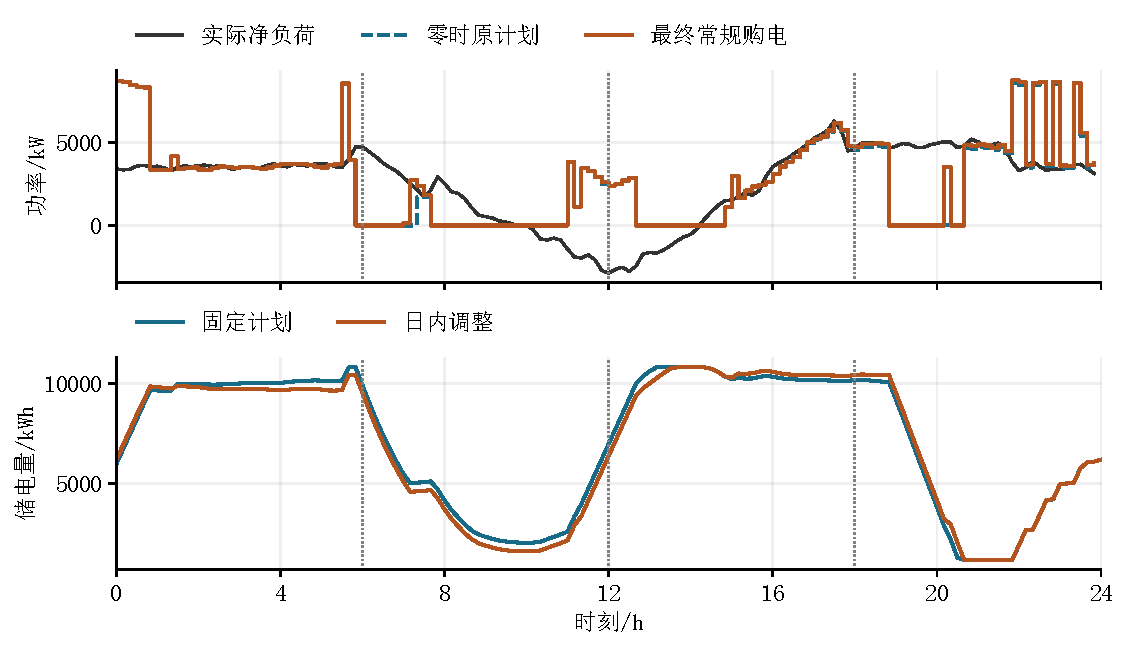
\includegraphics[width=\textwidth]{../outputs/figures/paper-q3-day.pdf}
 \caption{9月23日的日内购电调整与库存变化}\label{fig:q3-day}
\end{figure}
\FloatBarrier

\subsubsection{预报贡献与参数灵敏度}
各光伏来源先在相同1月区间选参，再从共同热启动和期初库存开始比较。融合方案比纯历史基准节省112379.91元，单用附件三则更贵，说明保留历史预测有助于降低本题的运行费用。完整费用见附录\ref{app:parameter-checks}表\ref{tab:q3-forecast}。某次新预报的作用，还需进一步控制调整机会等条件。

为判断是否需要其他时刻的预报，各组采用相同主参数、三次调整时刻、负荷修正及光伏插值起点，逐组改变允许读取的新预报；不读取时沿用最近可用的一次。各组共用1月热启动，随后按自身调度连续运行。表\ref{tab:hourly-marginals}列出每次单独撤去一项预报后的费用变化，八种组合的完整结果见附录\ref{app:parameter-checks}表\ref{tab:hourly-subsets}。
% Generated by scripts/build_paper_tables.py; do not edit by hand.
\par
\begin{table}[!htbp]
\centering
\caption{单独撤去一次新小时预报的条件费用差（元）}\label{tab:hourly-marginals}
\normalsize
\begin{tabular}{lrr}
\toprule
\multicolumn{1}{c}{撤去的预报} & \multicolumn{1}{c}{纯附件3} & \multicolumn{1}{c}{融合主策略} \\
\midrule
06点 & 53,593.3113 & 28,402.5518 \\
12点 & 74,628.9683 & 20,127.5241 \\
18点 & -0.1296 & -0.3123 \\
\bottomrule
\end{tabular}
\end{table}
\par

\FloatBarrier
读取全部新预报比均不读取节省17225.82元。撤去06或12点的新预报会增加费用，撤去18点后的变化仅$-0.31$元。因此，在本组参数下，前两次新预报有助于降低费用，18点的新预报收益很小。各次预报的影响随库存和后续计划相互关联，单项费用差不能直接相加。对照仍保留18点调整，可利用当时的负荷观测和库存变化重新安排购电。

分位扰动见表\ref{tab:q3-risk-sensitivity}。正式期$\alpha=0.50$的费用比主参数0.65低15787.50元，但紧急电量明显增大。1月评分较低的参数未必在后续月份同样省费，短期选参存在样本局限。主结果采用按1月费用选出的参数，全年扰动用于考察这一选择的影响。
\par
\begin{table}[!htbp]
\centering
\caption{问题三的分位参数扰动（2—12月）}\label{tab:q3-risk-sensitivity}
\normalsize
\begin{tabular}{lrrr}
\toprule
\multicolumn{1}{c}{$\alpha$} & \multicolumn{1}{c}{总费用/元} & \multicolumn{1}{c}{紧急购电/kWh} & \multicolumn{1}{c}{年末储电量/kWh} \\
\midrule
0.5 & 13,300,048.49 & 66,633.50 & 5,890.36 \\
0.65 & 13,315,835.99 & 25,862.57 & 5,987.72 \\
0.7 & 13,393,753.32 & 18,804.41 & 6,060.07 \\
0.9 & 14,101,446.70 & 2,544.90 & 6,507.64 \\
\bottomrule
\end{tabular}
\end{table}
\par

将日末预测恢复目标改为3000或9000\,kWh，结果见附录\ref{app:parameter-checks}表\ref{tab:q3-reserve}。目标较低时支出下降，热启动库存和期末库存也随之降低，因此费用变化同时反映了购电安排和储备电量的差异。
\FloatBarrier
逐笔成交不可撤回时，重新选参和优化的总费为\PaperValue{q3-per-trade-cost}\,元，仍比问题二低447673.33元，但节省少于主合约。附录\ref{sec:contracts}分别给出原调度重新计费及重新优化的结果，说明累计调整费的规则会影响方案收益。
\label{end:q3}
